% !TEX root = ../../main.tex
\subsection{系统闭环创新}

本作品实现了用户端、骑手端和管理员端的完整系统闭环。用户端支持注册登录、创建订单、Token 验证、订单通信、订单历史查看和溯源申请；骑手端支持订单查看、接单、进入订单通信房间和异常申请；管理员端支持登录认证、订单审计、消息摘要查看、Merkle Root 快照生成、完整性验证、三端摘要一致性验证和条件溯源处理。

从业务流程看，系统形成了如下闭环：

\begin{figure}[H]
    \centering
    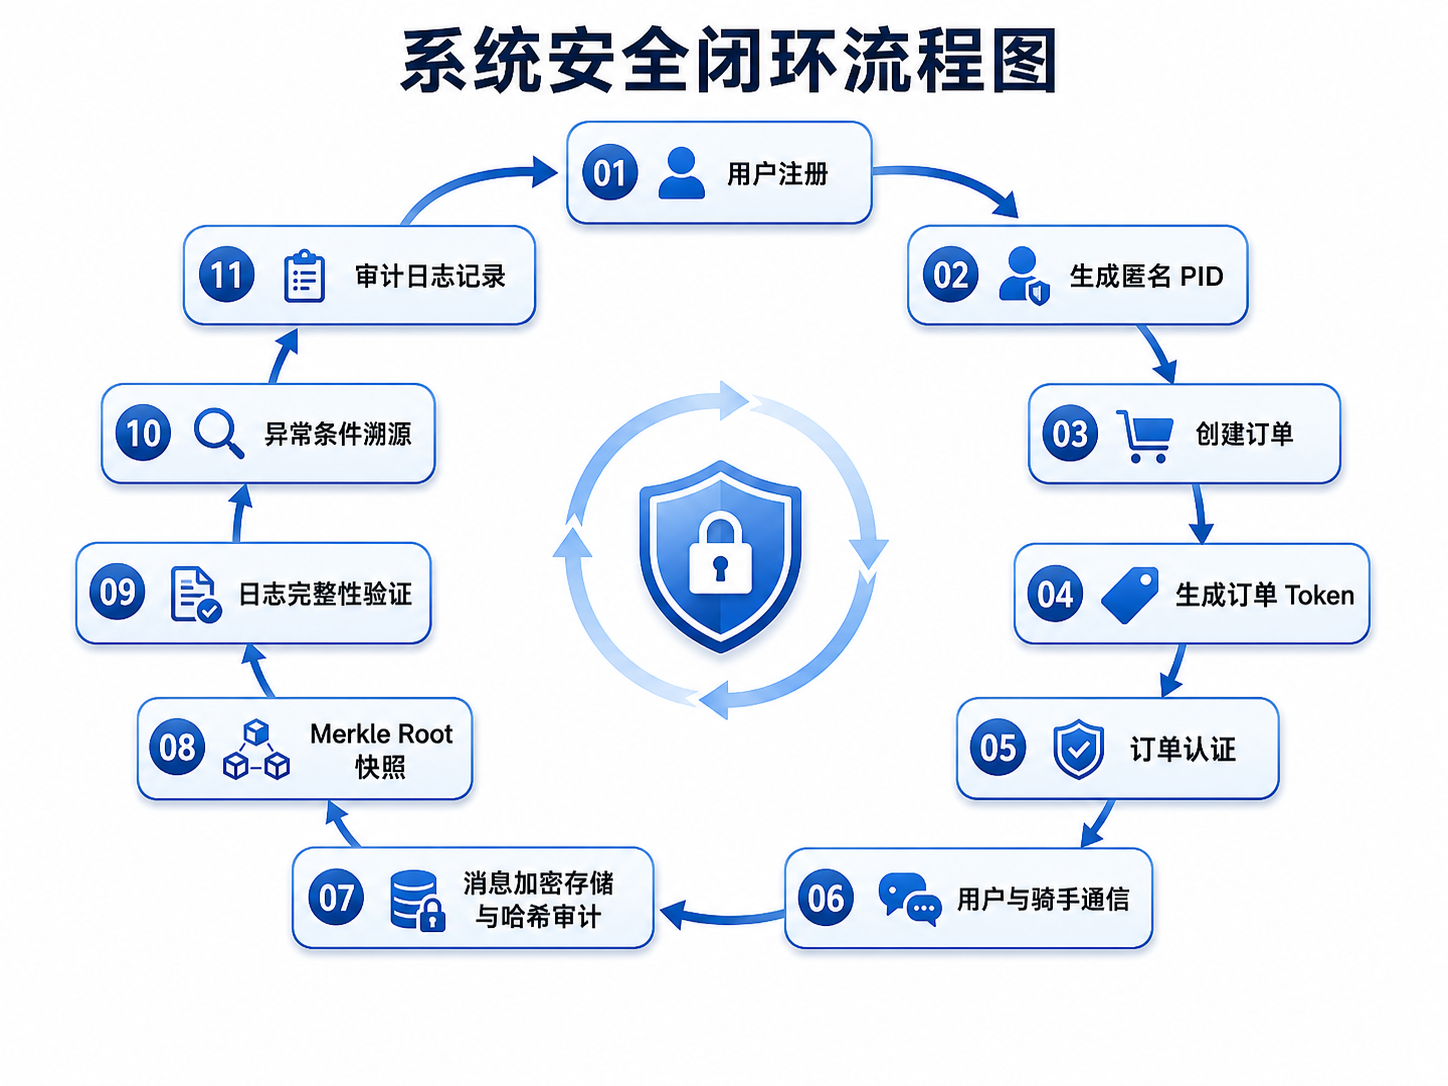
\includegraphics[width=0.8\textwidth]{content/chapter6/circle.png}
    \caption{系统安全闭环流程图}
    \label{fig:system-loop-flow}
\end{figure}

该闭环体现了本作品的工程完整性。系统不是仅实现一个单点功能，例如只生成 PID、只验证 Token 或只计算 Merkle Root，而是将多个安全机制嵌入到完整业务流程中。用户下单后的每一步操作都与后端安全控制相关联：订单创建绑定匿名身份，进入通信房间需要 Token 验证，消息发送触发加密存储和哈希计算，管理员验证依赖 Merkle Root 快照，异常处理通过订单号进行受控溯源。

这种闭环设计提高了作品的可展示性和可答辩性。评审可以从用户端、骑手端和管理员端分别观察系统运行效果，也可以通过正常通信、Token 篡改、日志篡改、权限校验和条件溯源等场景验证系统安全机制是否有效。相比仅停留在理论方案层面的设计，本作品提供了可运行、可交互、可演示的系统原型。
